A tally was made of all the subsystems included in the spacecraft. First a division can be made by distinguishing between the subsystems pertaining to the crew module and those included in the \gls{hiad}. This division is shown in figure \ref{fig:subsystems}. Also shown in figure \ref{fig:subsystems} are all the subsystems included in the crew module and decelerator.
\begin{figure}[h]
	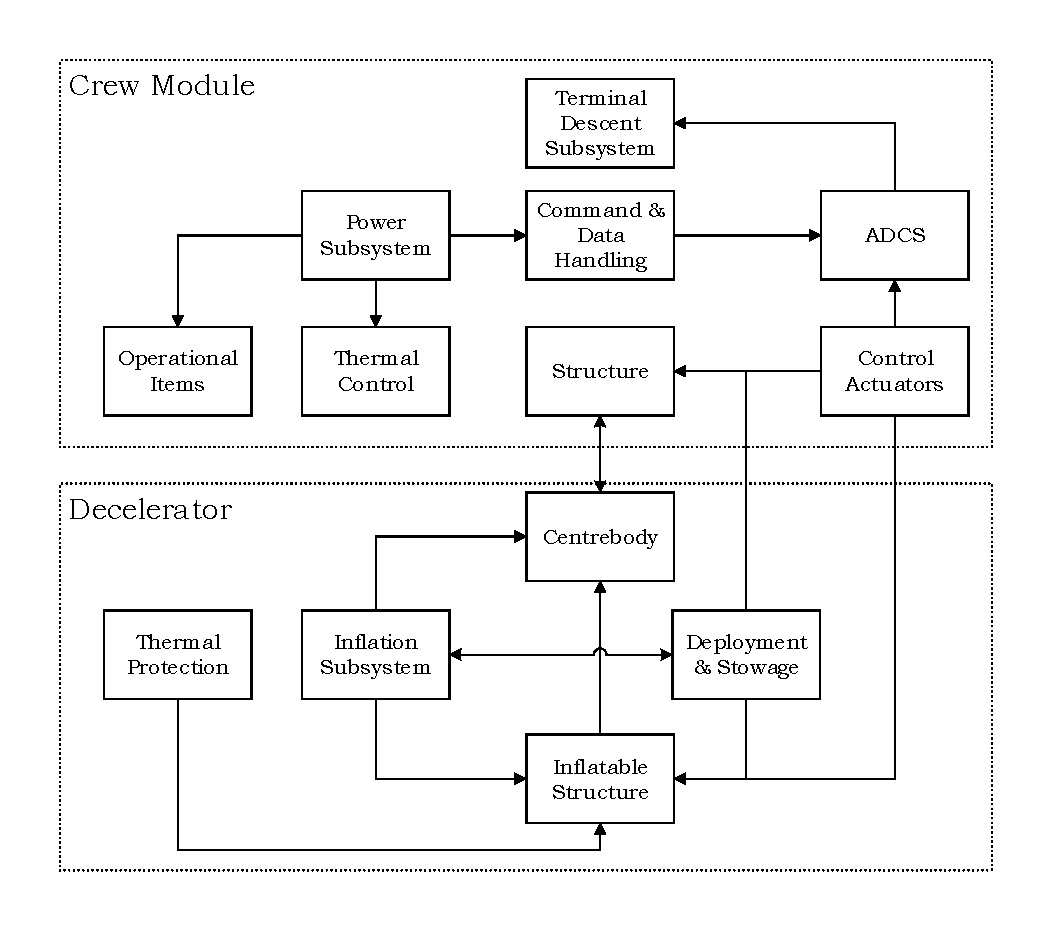
\includegraphics[width=0.95\textwidth]{./Figure/subsystem_breakdown/hardware_structure.pdf}
	\caption{Spacecraft subsystem breakdown}
	\label{fig:subsystems} 
\end{figure}
%There exist some links between several of the subsystems. The \gls{tps} needs to protect the inflatable structure, centerbody, actuators and crew module. 
%
%** relation tussen inflation system, deployment en inflatable structure **
%
%** relation tussen inflatable structure en centerbody**
%
%** relation betwussen locaties actuators \& type control system (thrusters, flaps, cg offset) **
%
%** relation between actuators \& ADCS van crew module **
%
%** relatie tussen thermal control \& operational items van crew module**
%

As can be seen from figure \ref{fig:subsystems} connections exist between several of the subsystems, both confined to the decelerator and crew module and between them. In the decelerator the inflation system and deployment \& stowage systems are closely related with the inflatable structure. The former two are required in order to activate the stowed inflatable structure to fulfil its mission. While decelerating the \acrlong{tps} has to protect the inflatable structure from the intense heat produced by aerodynamic forces. 